
\documentclass[12pt]{article}
\usepackage{geometry} 
\usepackage{setspace}
\usepackage[italian]{babel}
\usepackage[utf8]{inputenc}
\usepackage{color}
\usepackage{indentfirst}
\usepackage{listings}
\usepackage{graphicx}
\usepackage[dvipsnames]{xcolor}
\usepackage{url}

\geometry{a4paper} 

\lstnewenvironment{codice}
{\lstset{basicstyle=\ttfamily, columns=fullflexible,
keywordstyle=\color{ForestGreen}\bfseries, commentstyle=\color{MidnightBlue}, stringstyle=\color{BrickRed},
language=Python,
numbers=left, numberstyle=\tiny,
stepnumber=2, numbersep=5pt, frame=single,breaklines=True}}{}

\title{\textbf{EasYE TRACKING}}
\author{Giada Colella \and Chiara Coletti}
\date{15/07/2016} 


\begin{document}
	

\begin{figure}
\centering
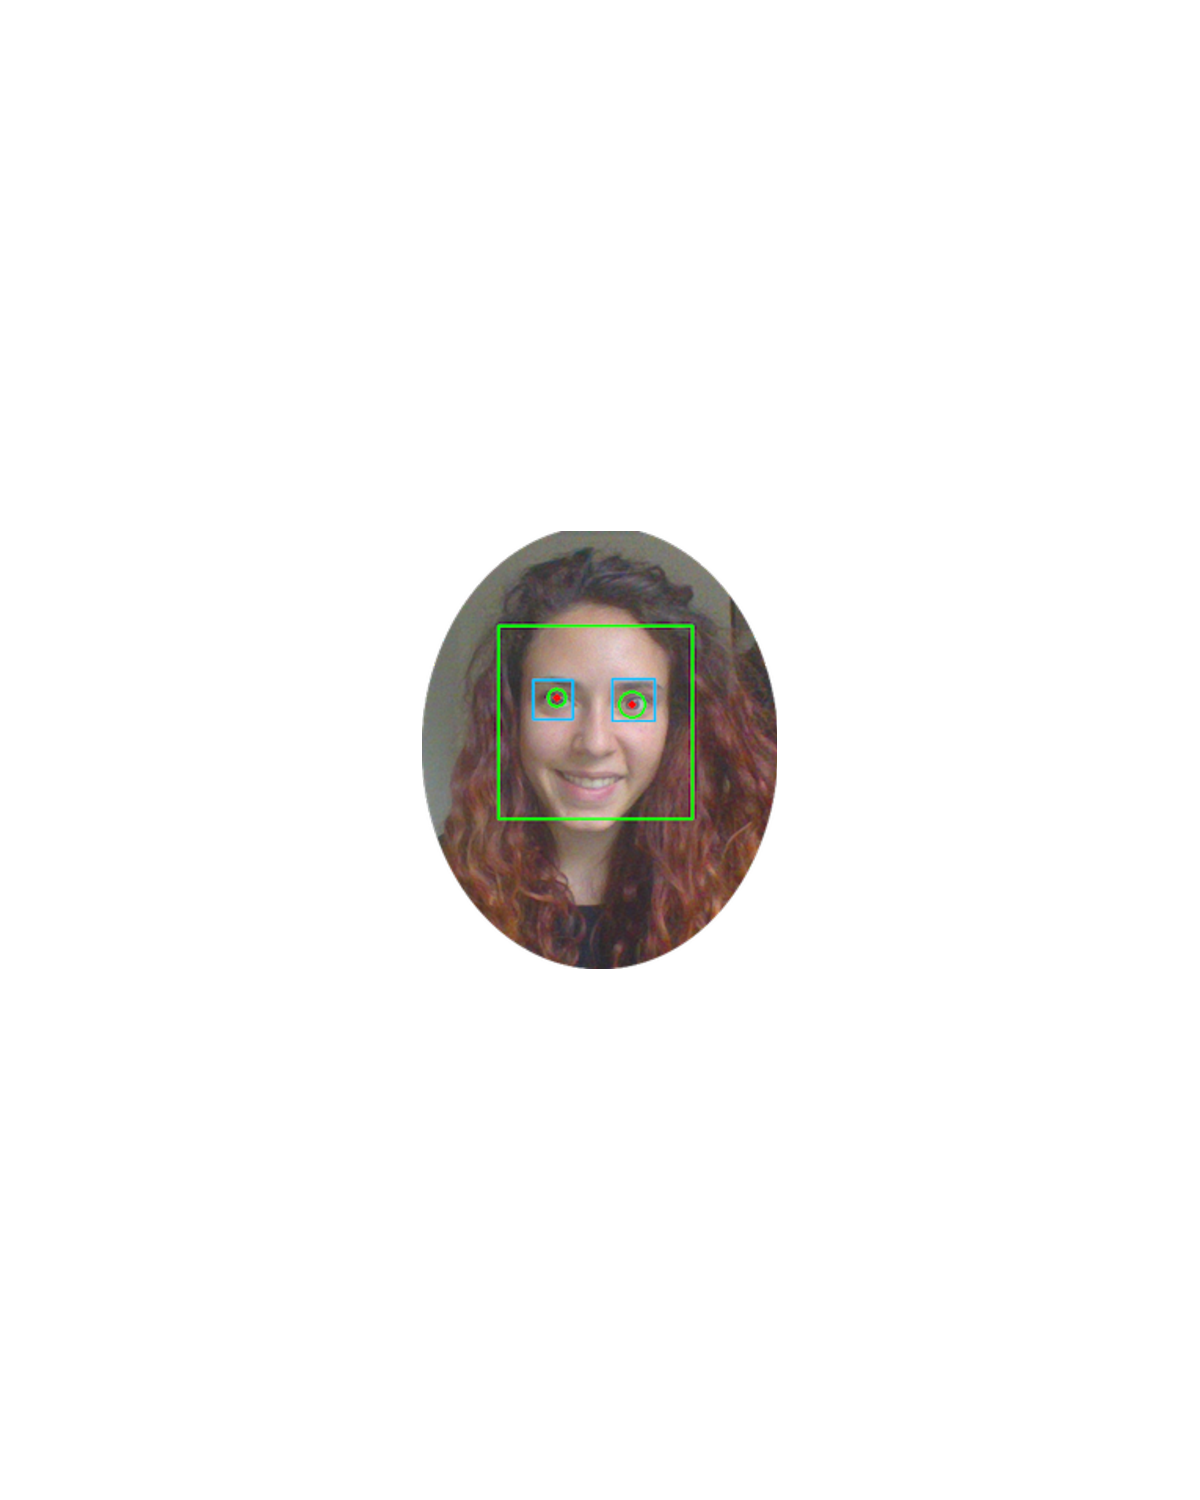
\includegraphics[width=6cm,height=7.2cm]{im2}%
\qquad\qquad
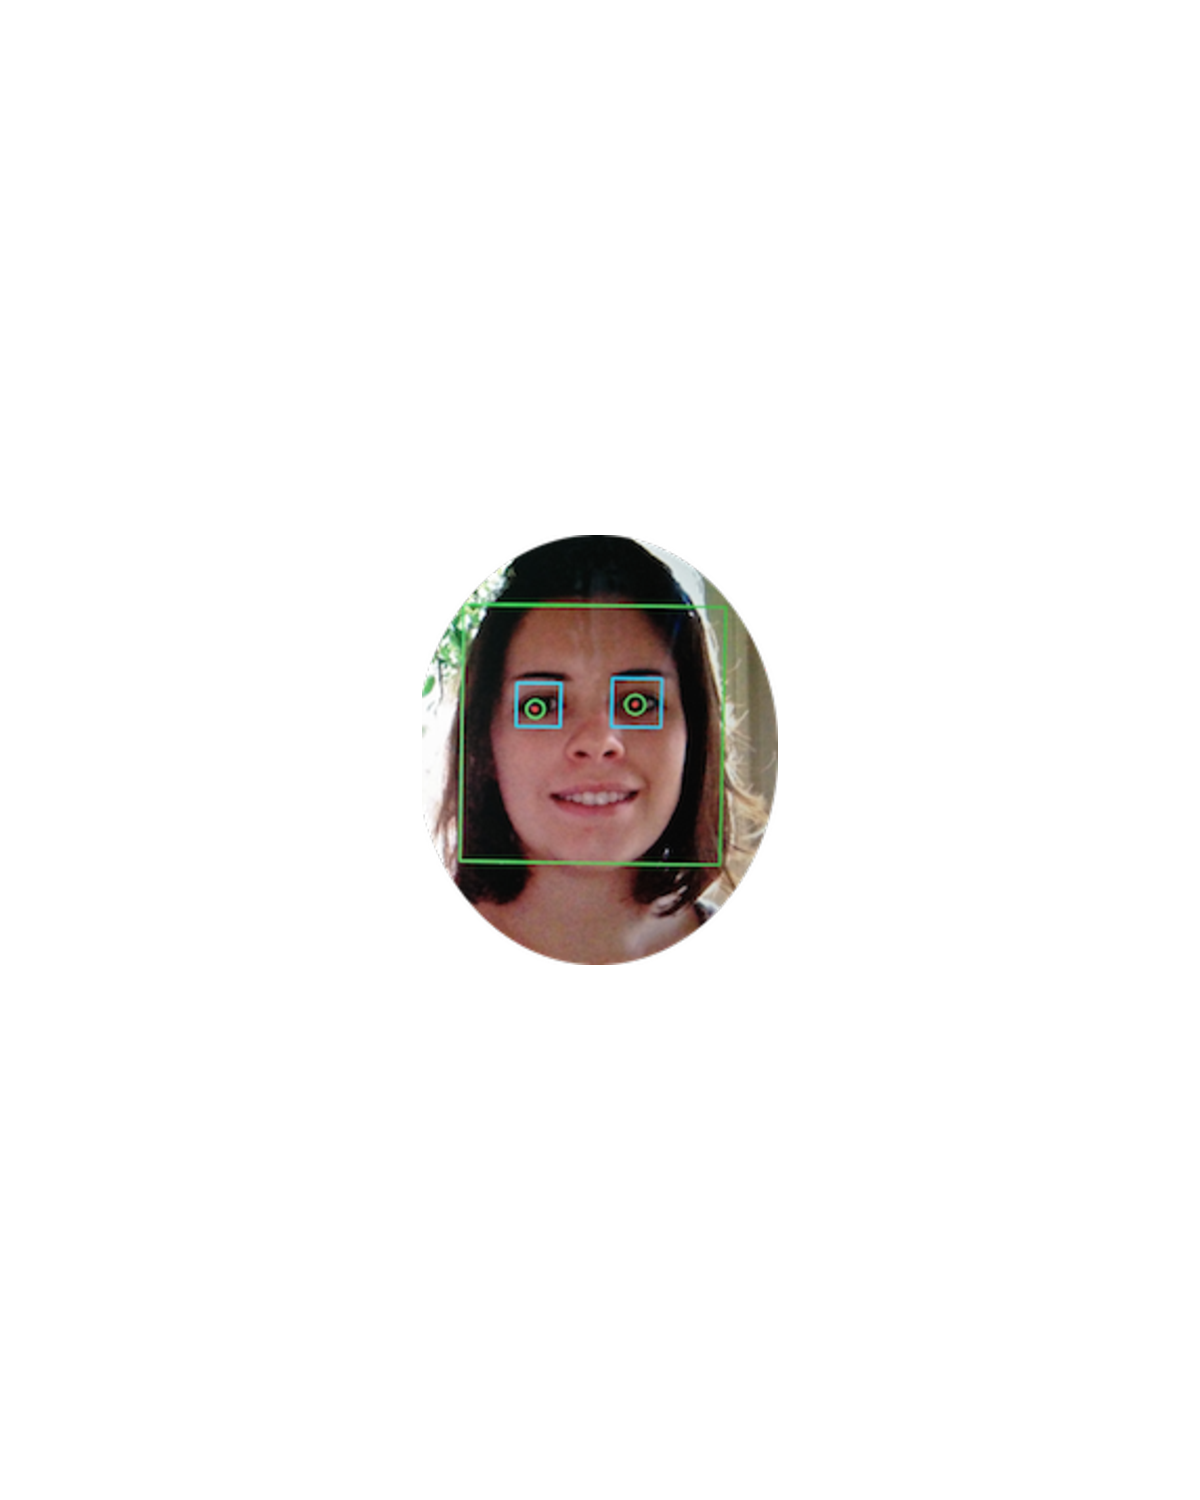
\includegraphics[width=6.1cm,height=7.25cm]{im}
\end{figure}

\maketitle
\pagebreak

\tableofcontents

\pagebreak

\begin{abstract}
	L' \textbf{Eye tracking} \`e un complesso processo di misurazione del punto di fissazione oculare. I vantaggi che derivano dall'utilizzo di questa tecnica sono molteplici: a partire da indagini statistiche di mercato fino al miglioramento della comunicazione uomo/macchina.\\
	Quando si guarda qualcosa gli occhi si spostano almeno 3/4 volte al secondo tramite movimenti detti "saccadi" che durano circa un decimo di secondo, mentre le fissazioni durano da 2 a 4 decimi di secondo. Questi movimenti continui sono alla base dei meccanismi del sistema visivo... e dell' Eye tracking. \\
	Sul mercato esistono diverse tipologie di eye tracker come VideoTracker (una telecamera registra i movimenti oculari dell'utente rispetto allo schermo) o InfraredTracker (strumento che studia la riflessione dei raggi infrarossi da parte della pupilla).
\end{abstract}
\pagebreak
\section{Introduzione}
Il progetto \textbf{EasYe Tracking} si pone nella prima fase di realizzazione di un eye tracker. Ha come scopo lo studio del movimento dell'occhio. Partendo da un video, si cerca di individuare l'occhio e di tracciarne il movimento. Punto focale della ricerca \`e stato il riconoscimento della posizione del centro dell'iride rispetto alla finestra video. 
\\In questo documento viene affrontato lo studio dell' Eye tracking tramite due aprocci differenti: il codice che viene presentato  al punto \textbf{4 "Codice completo"}, permette di riconoscere la posizione del'occhio nella finestra video. Non da dunque alcuna informazione riguardante il movimento relativo del'iride rispetto al volto.
Nella sezione \textbf{5 "Per migliorare"}, invece, viene presentato un secondo approccio, pi\`u specifico per il problema Eye Tracking. Presa l'immagine in ingresso dalla telecamera, vengono studiate le modifiche di colore della zona occhi e, a partire da quelle, il programma fornisce indicazioni riguardanti il movimento oculare relativo al volto.
\\Il progetto \`e stato sviluppato usando {\textbf{"Python"} come linguaggio di programmazione. Il primo passo per la realizzazione del progetto \`e stato installare la libreria libera \textit{\textbf{Opencv}}. Opencv permette, tra le altre funzioni, di manipolare immagini, inseguire oggetti (Object Tracking) o effettuarne un riconoscimento (Pattern Recognition). Il riconoscimento di volti ed occhi \`e stato realizzato mediante l'algoritmo "Cascade Classification". Prima di operare, dunque, è stato necessario importare i file classificatori (o "haarcascades") nella cartella di lavoro.

	\subsection{Cosa sono le Haarcascades}
	Il riconoscimento di oggetti in un'immagine o in un video \`e uno dei principali argomenti trattati in questo progetto. \\
	Il metodo di riconoscimento che \`e stato scelto \`e l' \textbf{Haarcascades classification}. \`E un algoritmo basato sull'applicazione a cascata di funzioni classificatrici, introdotto per la prima volta nel 2001. 
	Dapprima un classificatore è addestrato con qualche centinaia di immagini campione di un particolare oggetto (immagini positive) e altri immagini campione di sfondo (immagini negative) tutte portate alla stessa dimensione. \\ Successivamente il classificatore viene applicato alla regione di interesse (ROI, region of interest) dell'immagine input. La funzione ritorna "1" in caso di matching tra oggetti tra la ROI il classificatore, "0" altrimenti. \\
	La parola "cascade" nel nome dell'algoritmo significa che il classificatore finale \`e il risultato di varie applicazioni seriali di classificatori pi\`u semplici che si interrompono quando tutte hanno dato esito positivo o quando in un solo passaggio la ROI \`e stata rigettata.
\pagebreak

\section{Dallo Pseudocodice...}
Abbiamo ritenuto utile suddividere il nostro progetto in vari step:
\begin{enumerate}
	\item \label{primo}\textcolor{Plum}{Acquisizione video e analisi frame by frame}
	\item \label{secondo} \textcolor{Plum}{Conversione dei frame acquisiti in scala di grigi}
	\item \label{terzo} \textcolor{Plum}{Riconoscimento del volto}
	\item \label{quarto}\textcolor{Plum}{Riconoscimento degli occhi}
    \item \label{quinto}\textcolor{Plum}{Riconoscimento cerchi nell'area occhi}
    \item \label{sesto}\textcolor{Plum}{Rappresentazione del movimento oculare}
    \item \label{settimo}\textcolor{Plum}{Generazione video e chiusura programma}
\end{enumerate}

\pagebreak
\section{...Al codice}
\vspace{1cm}
Importiamo le librerie oportune, introduciamo i parametri che ci torneranno utili nella stesura del codice ed importiamo le Haarcascades che userem per il riconoscimento di volto e occhi.
\vspace{1cm}
\begin{codice}
%matplotlib inline
import matplotlib.pyplot as plt
import cv2
import numpy as np

sc_fct = 1.1              
min_neigh = 5             
min_size_f = (30,30)      
min_size_e = (10,10)        
mindist_c=30               
dp_c=1                   
param1_c=60               
param2_c=20              
minr_c=5                
maxr_c=15                 


faceCascade=cv2.CascadeClassifier("haarcascade_frontalface_default.xml")
eyeCascade=cv2.CascadeClassifier("haarcascade_eye.xml")
\end{codice}

\vspace{2cm}
\ref {primo} \underline{\textbf{\textcolor{Plum}{Acquisizione video e analisi frame by frame}}}

\vspace{1cm}
Abbiamo importato il video dalla webcam, rinominato la finestra video e salvato in "frame" gli elementi su cui poi andremo a lavorare. L'ultima operazione vine inserita all'interno di un ciclo while che verrà interrotto solo al termine dell'esecuzione dell'intero programma.

\vspace{1cm}
    \begin{codice}
video_capture = cv2.VideoCapture(0)
cv2.namedWindow("Face and eyes")
    
while True:
    ret, frame = video_capture.read()
    \end{codice}

\vspace{1cm}
    
 Definisco x\_dim e y\_dim come le dimensioni del video in entrata. Saranno utili in seguito. 
 
 \vspace{1cm}  
    
\begin{codice}
x_dim=video_capture.get(3)
y_dim=video_capture.get(4)
\end{codice}
\vspace{2cm}

  
  
\ref {secondo} \underline{\textbf{\textcolor{Plum}{Conversione dei frame acquisiti in scala di grigi}}}
 \vspace{1cm}
 
 
 Applichiamo la funzione 'cvtColor' specificando il tipo di conversione da eseguire (in questo caso convertiamo da una figura a colori ad una a scala di grigi mediante il comando cv2.COLOR\_BGR2GRAY). La funzione viene applicata a 'frame' ovvero la zona di memoria in cui vengono salvati i singoli frame del video.
 \vspace{1cm}
 
\begin{codice}
	gray = cv2.cvtColor(frame, cv2.COLOR_BGR2GRAY)
\end{codice}

 \vspace{2cm} 	
  	
  
\ref {terzo} \underline{\textbf{\textcolor{Plum}{Riconoscimento del volto}}}
\vspace{1cm}

Applichiamo la funzione 'detectMultiscale' e utilizziamo le cascaspecificando il tipo di conversione da eseguire (in questo caso convertiamo da una figura a colori ad una a scala di grigi mediante il comando cv2.COLOR\_BGR2GRAY). La funzione viene applicata a 'gray' ovvero la zona di memoria in cui abbiamo salvato i risultati della conversione dei vari frame in scala di grigi. Salviamo l'output della funzione (una lista di quattro elementi: coordinata x e coordinata y del vertice superiore sinistro del rettangolo, base e altezza) in "faces".  
\vspace{1cm}

\begin{codice}
    faces = faceCascade.detectMultiScale(       
        gray,
        scaleFactor=sc_fct,
        minNeighbors=min_neigh,
        minSize=min_size_f
        )
\end{codice}
\vspace{1cm}

Tracciamo i rettangoli attorno ai volti riconosciuti mediante la funzione 'rectangle'.
\vspace{1cm}

 \begin{codice}
    for (x, y, w, h) in faces:
            cv2.rectangle(frame,(x, y), (x+w, y+h), (0, 255, 0), 2)
\end{codice}

\vspace{2cm}	  	
  	
\ref {quarto} \underline{\textbf{\textcolor{Plum}{Riconoscimento degli occhi}}}

\vspace{1cm}

Definisco nuove aree di lavoro: rappresentano la stessa area (limitata alla metà superiore del volto), la prima è in scala di grigi, la seconda a colori.

\vspace{1cm}


 \begin{codice}
            roi_gray=gray[y:y+h/2,x:x+w]
            roi_color=frame[y:y+h/2,x:x+w]

\end{codice}

\vspace{1cm}


Applichiamo nuovamente la funzione 'detectMultiscale'. Questa volta la funzione viene applicata a 'roi\_gray'.Salviamo l'output della funzione in "eyes".
\vspace{1cm}
 
 \begin{codice}
             eyes= eyeCascade.detectMultiScale(         
                 roi_gray,
                 scaleFactor=sc_fct,
                 minNeighbors=min_neigh,
                 minSize=min_size_e
                 )  
 \end{codice}
\vspace{1cm}

Tracciamo i rettangoli attorno agli occhi riconosciuti mediante la funzione 'rectangle'.
\vspace{1cm}
 
 \begin{codice}
            for (ex, ey, ew, eh) in eyes:
                cv2.rectangle(roi_color, (ex, ey), (ex+ew, ey+eh), (255, 191, 0), 2)
\end{codice}

\vspace{2cm}
  	 	
 \ref {quinto} \underline{\textbf{\textcolor{Plum}{Riconoscimento cerchi nell'area occhi}}}
 
 \vspace{1cm} 	
 
 
 Definisco nuove aree di lavoro: rappresentano la stessa area (limitata ai rettangoli degli occhi riconosciuti), la prima è in scala di grigi, la seconda a colori.
 \vspace{1cm}
 \begin{codice}
                roi_gray2=roi_gray[ey:ey+eh,ex:ex+ew]
                roi_color2=roi_color[ey:ey+eh,ex:ex+ew]

\end{codice}

\vspace{1cm}

Applichiamo la funzione 'HoughCircles' per il riconoscimento degli occhi nell'area inserita come input (roi\_gray2). Salviamo l'output della funzione (una lista di tre elementi: coordinata x, coordinata  e raggio del cerchio riconosciuto) in "circles".
\vspace{1cm}

\begin{codice}
                circles = cv2.HoughCircles(roi_gray2,cv2.HOUGH_GRADIENT,dp=dp_c,minDist=mindist_c,
                            param1=param1_c,param2=param2_c,minRadius=minr_c,maxRadius=maxr_c)

\end{codice}
\vspace{1cm}

Introduciamo la condizione che ci permette di "bypassare" i frame in cui non viene riconosciuto alcun cerchio. Nel caso in cui, invece, il cerchio venga riconosciuto, 'circles' viene trasformato in un ato di tipo intero.
\vspace{1cm}
\begin{codice}
                if(circles==None):
                    continue
                else:
                     circles = np.uint16(np.around(circles[0,:]))
\end{codice}

\vspace{1cm}

Tracciamo i cerchi e il loro centro.
\vspace{1cm}

 \begin{codice}
                  for (x_c,y_c,r) in circles:
                    cv2.circle(roi_color2,(x_c,y_c),r,(0,255,0),2)
                    cv2.circle(roi_color2,(x_c,y_c),2,(0,0,255),3)
\end{codice}

  \vspace{2cm}	 				
  	 				
  	 				
  	 				
\ref {sesto} \underline{\textbf{\textcolor{Plum}{Rappresentazione del movimento oculare}}}
\vspace{1cm}


Introduco uno scatterplot di dimensioni (x\_dim e y\_dim) pari alle dimensioni del video in cui visualizzo il centro di cerchio trovato. I punti hanno una trasparenza tale da permettere di osservare le zone dello scatterplot più dense di punti: ovvero quelle zone in cui lo il centro dell'iride è stato più presente.
\vspace{1cm}

\begin{codice}
                    plt.scatter(x+ex+x_c,y+ey+y_c, s=100, c='r',alpha=0.3)
                    plt.axis([0,x_dim,0,y_dim])
                    plt.draw()
\end{codice}
\vspace{1cm}
 Si ottiene un output di questo tipo:
\\
\\

\begin{figure}[htbp]
\centering
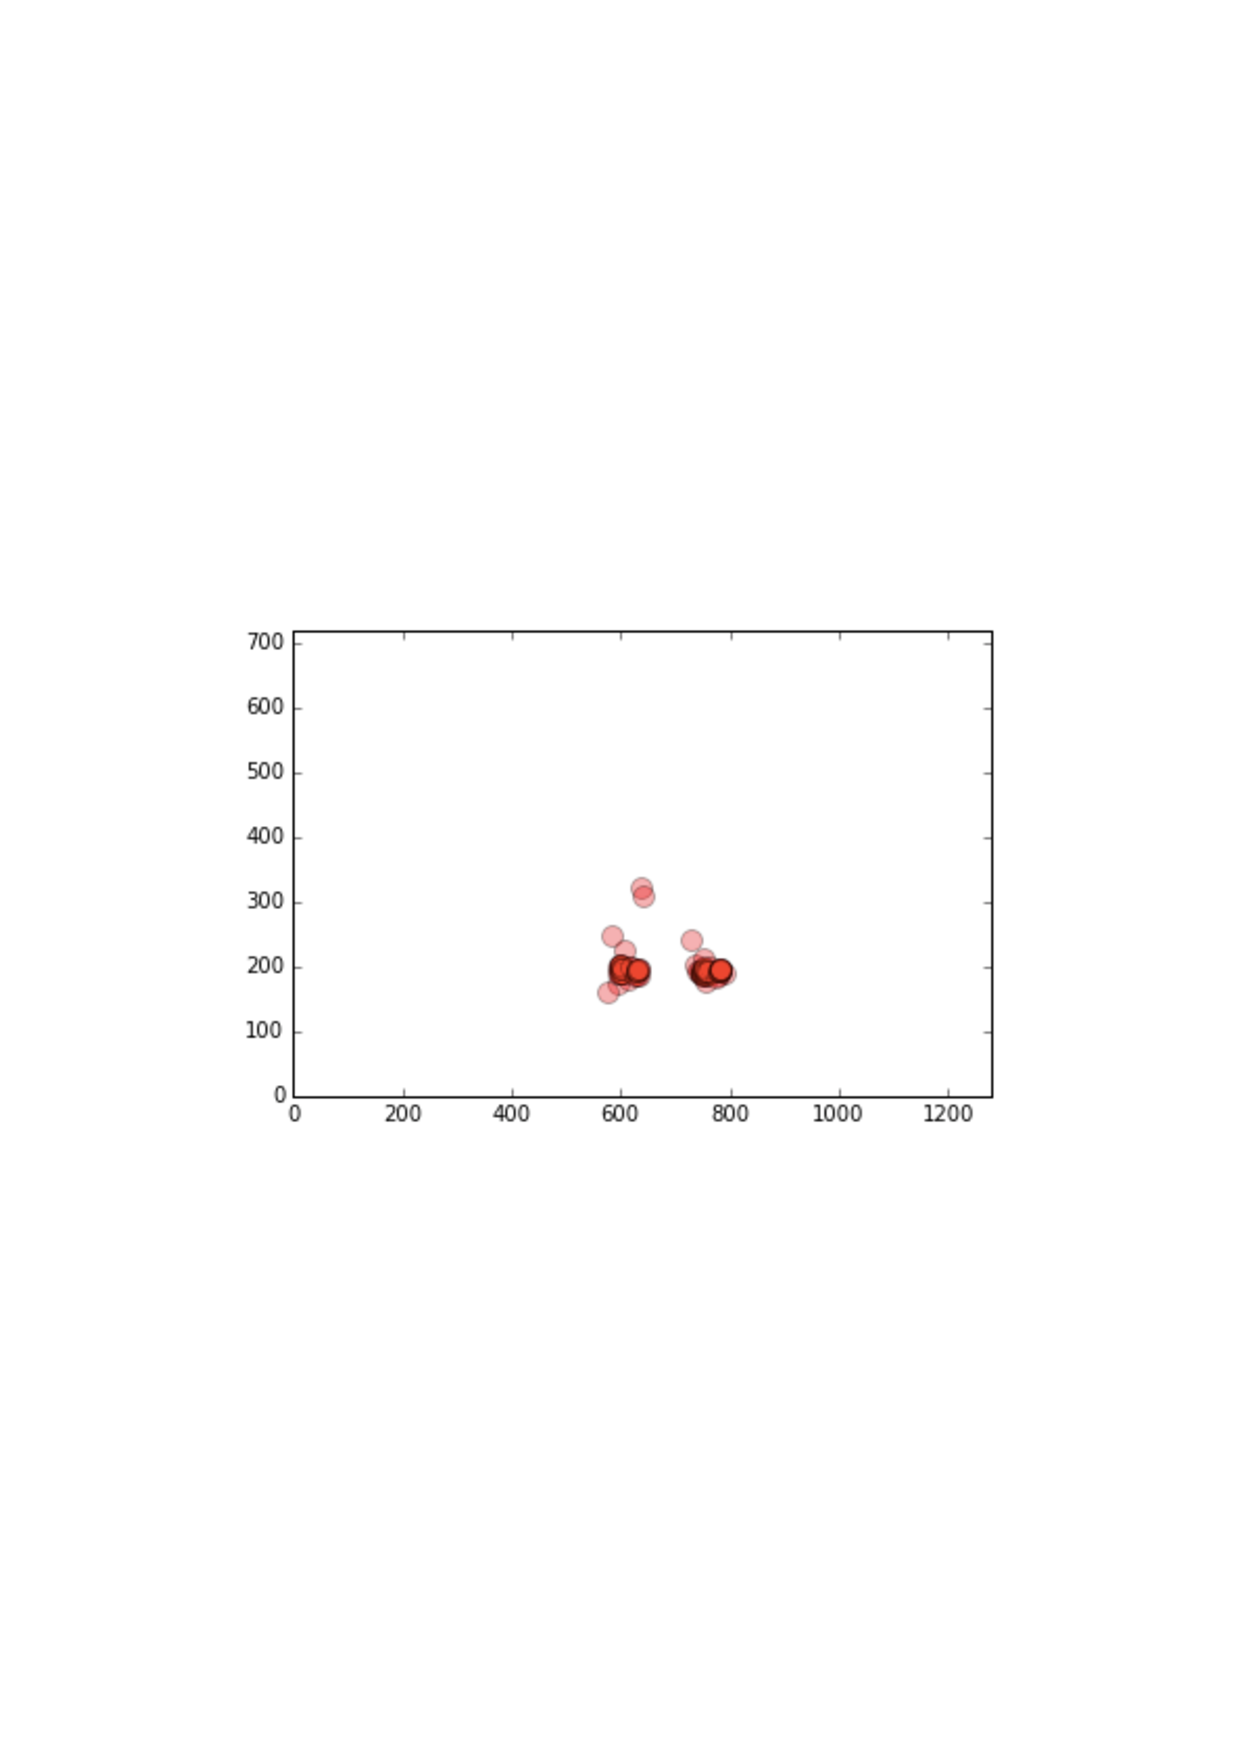
\includegraphics{scatter}
\caption{Esempio scatterplot}
\end{figure}
\vspace{1cm}


\ref {settimo} \underline{\textbf{\textcolor{Plum}{Generazione video e chiusura programma}}}
\vspace{1cm}

Mostriamo il video. In 'frame' saranno state apportate le modifiche delle varie aree di interesse. Nel video saranno dinque mostrati i rettangoli dei volti e degli occhi riconosciuti e i cerchi trovati all'interno dei rettangoli degli occhi.
\vspace{1cm}
 \begin{codice}
    cv2.imshow('Face and eyes', frame)
\end{codice}
\vspace{1cm}

Interuzione del ciclo iniziato al momento della cattura dei frame e chiusura della finestra video quando viene premuto il tasto 'Esc'.
\vspace{1cm}
\begin{codice}
    if cv2.waitKey(1)==27:
        break

\end{codice}
\vspace{1cm}

Chiusura di tutte le finestre.
\vspace{1cm}

\begin{codice}
video_capture.release()
cv2.destroyAllWindows()

\end{codice}

   
\pagebreak  	 					

\section{Codice completo}
\begin{codice}

%matplotlib inline
import matplotlib.pyplot as plt

import cv2
import numpy as np

#Parameters setting:
sc_fct = 1.1              #scaling factor
min_neigh = 5             #minimum number of neighbours to identify an area as the specific object
min_size_f = (30,30)      #smallest face dimensions accepted
min_size_e = (10,10)      #smallest eye dimension accepted  
mindist_c=30               #minimum distance between circles' centers
dp_c=1                    #accumulator resolution factor
param1_c=60               #specific parameter of the Hough Gradient detection method 
param2_c=20              #specific parameter of the Hough Gradient detection method
minr_c=5                  #minimum circle radius accepted
maxr_c=15                  #maximum circle radius accepted




#Loading the cascade classifier files
faceCascade = cv2.CascadeClassifier("haarcascade_frontalface_default.xml")
eyeCascade=cv2.CascadeClassifier("haarcascade_eye.xml")

#Capturing the video from the webcam and opening a window to display it
video_capture = cv2.VideoCapture(0)
cv2.namedWindow("Face and eyes")

#Saving the window dimensions
x_dim=video_capture.get(3)
y_dim=video_capture.get(4)

while True:
    #Capturing frames from the video
    ret, frame = video_capture.read()
    
    #Converting the image from colour to grayscale
    gray = cv2.cvtColor(frame, cv2.COLOR_BGR2GRAY)
    
    #Using the cascade classifier to identify faces in the video
    faces = faceCascade.detectMultiScale(       
        gray,
        scaleFactor=sc_fct,
        minNeighbors=min_neigh,
        minSize=min_size_f
        )
    #detectMultiscale function returns a list of rectangles described by the upper left vertex and the two dimensions

    #Drawing rectangles recognised by the detectMultiscale function
    for (x, y, w, h) in faces:
            cv2.rectangle(frame,(x, y), (x+w, y+h), (0, 255, 0), 2)
            
            #Defining new regions of interest
            roi_gray=gray[y:y+h/2,x:x+w]
            roi_color=frame[y:y+h/2,x:x+w]
        
        #Using the cascade classifier to identify eyes within the new ROI just defined
            eyes= eyeCascade.detectMultiScale(         
                 roi_gray,
                 scaleFactor=sc_fct,
                 minNeighbors=min_neigh,
                 minSize=min_size_e
                 )


            #Drawing rectangles returned by the detectMultiscale function
            for (ex, ey, ew, eh) in eyes:
                cv2.rectangle(roi_color, (ex, ey), (ex+ew, ey+eh), (255, 191, 0), 2)
            
                #Defining new regions of interest 
                roi_gray2=roi_gray[ey:ey+eh,ex:ex+ew]
                roi_color2=roi_color[ey:ey+eh,ex:ex+ew]
                
                #Applying HoughCircles function to identify iris and pupil in the filtered image (HOUGH_GRADIENT is the method used)
                circles = cv2.HoughCircles(roi_gray2,cv2.HOUGH_GRADIENT,dp=dp_c,minDist=mindist_c,
                            param1=param1_c,param2=param2_c,minRadius=minr_c,maxRadius=maxr_c)
                #The function returns a list of circles described by the centre coordinates and the radius
                    
                #Checking validity of the detected objects    
                if(circles==None):
                    continue
                else:
                #Coverting floats to integers to make values usable by the circle function
                  circles = np.uint16(np.around(circles[0,:]))
            
                  #Drawing identified circles in the video
                  for (x_c,y_c,r) in circles:
                    cv2.circle(roi_color2,(x_c,y_c),r,(0,255,0),2)
                    cv2.circle(roi_color2,(x_c,y_c),2,(0,0,255),3)
                           
                    #Plotting a scatterplot with the eyes pupils' position through time
                    plt.scatter(x+ex+x_c,y+ey+y_c, s=100, c='r',alpha=0.3)
                    plt.axis([0,x_dim,0,y_dim])
                    plt.draw()
    
    #Showing the filtered image and the webcam video
    cv2.imshow('Face and eyes', frame)
    
    
    #Breaking the while cicle when 'return' is pressed
    if cv2.waitKey(1)==27:
        break
    
#Closing al windows and turning webcams off
video_capture.release()
cv2.destroyAllWindows()
\end{codice}

\pagebreak
\section{Per migliorare}
Il codice cos\`i proposto permette di tracciare in maniera consistente i movimenti degli occhi rispetto alla totalit\`a dello schermo. Ma l'eyetracking va oltre. \\
Il vero punto d'arrivo \`e osservare i movimenti oculari rispetto al capo. A questo proposito abbiamo implementato il codice proposto nella sezione precedente mediante un algoritmo che permetta di studiare il movimento dell'iride studiando le variazioni di colore nella zona oculare.\\
Lo pseudocodice e il codice qui proposti hanno i primi quattro punti in comune con il codice già visto.

\subsection{Dallo pseudocodice...}
\begin{enumerate}
    \item \label{cinque}\textcolor{Plum}{Studio del movimento oculare}
    \begin{enumerate}
    	\item \label{1} \textcolor{Plum}{Rappresentazione dell'immagine in bianco e nero}
    	\item \label{2} \textcolor{Plum}{Studio del movimento delle zone di colore}
    \end{enumerate}
    \item \label{sei}\textcolor{Plum}{Rappresentazione del movimento oculare}
\end{enumerate}

\subsection{...Al codice}
\vspace{1cm} Prima di procedere \`e necessario introdurre tre funzioni che ci torneranno utili nel corso della stesura del programma. 

\vspace{1cm} La funzione \textbf{'calc\_min\_max'} permette di trovare il valore massimo e minimo di grigio dell'immagine inviata in ingresso. Ha come parametri d'ingresso un'immagine e le sue due dimensioni. La funzione ritorna due valori: min\_gray e max\_gray.
\\
\\


 \begin{codice}
 	def calc_min_max(matr,ew,eh):
 	min_gray=255
 	max_gray=0
 	a=0
 	b=0
 	for i in range(0,eh):
 	   for j in range(0,ew):
 	      if (matr[i][j]>max_gray):
 	         max_gray=matr[i][j]
 	      if (matr[i][j]<min_gray):
 	         min_gray=matr[i][j]
 	return min_gray,max_gray
 \end{codice}

\vspace{1cm} La funzione \textbf{'calc\_mean'} permette di trovare le coordinate x e y del punto che rappresenta la media del bianco nel'immagine. Per ottimizzare l'utilizzo di questa funzione \`e necessario che sull'immagine in ingresso sia stata precedentemente applicata una trasformazione che ne esalti il contrato sino a renderla un'immagine in soli bianco e nero. I parametri in ingresso della funzione sono: l'immagine input e le sue dimensioni. L'output della funzione è costituito dalle coordinate del punto di media.
\\
\\


\begin{codice}
def calc_mean(matr,ew,eh):
cont=0
a=0
b=0
for i in range(0,eh):
   for j in range(0,ew):
      if (matr[i][j]==255):
         a=a+i;
         b=b+j;
         cont=cont+1;
      if cont>0:
         c=float(a/cont)
         d=float(b/cont)
return c,d

\end{codice}

\vspace{1cm} La funzione \textbf{'leds\_on'} permette di accendere due dei quattro led che verranno tracciati nel corso dell'esecuzione del programma a seconda della posizione del punto di media del bianco rispetto all'immagine. Ha come parametri in ingresso le coordinate del punto media del bianco e le dimensioni dell'immagine sulla quale era stata precedentemente applicata 'calc\_mean'.
\\
\\
\begin{codice}
	#Initialising color variables for leds (BGR format)
	col_up=(0,0,0)
	col_down=(0,0,0)
	col_left=(0,0,0)
	col_right=(0,0,0)
	
def leds_on(x_m,y_m,ew,eh):
global col_up
global col_down
global col_left
global col_right
if (x_m>ew/2):
    col_down=(0,255,0)
	col_up=(0,0,0)
else:
	col_up=(0,255,0)
	col_down=(0,0,0)
if (y_m>eh/2):
	col_right=(0,255,0)
	col_left=(0,0,0)
else:
	col_left=(0,255,0)
	col_right=(0,0,0)
\end{codice}

\vspace{2cm}

\ref {cinque} \underline{\textbf{\textcolor{Plum}{Studio del movimento oculare}}}
\\
\\
\ref{1} \textcolor{Plum}{Rappresentazione dell'immagine in bianco e nero}

 \vspace{1cm} Dopo aver applicato la funzione 'calc\_min\_max', utilizzo il valore massimo di grigio trovato (che equivale al pixel più chiaro dell'immagine) per definire una delle due soglie di grigio. Le due soglie vengono poi inserite come input nella funzione 'inRange' utile per evidenziare (bianco) tutti i pixel dell'immagine input i cui colori sono al'interno della soglia impostata. Attraverso l'uso della funzione 'calc\_min\_max' \`e possibile effettuare uno studio adattativo dei valori di grigio sui vari frame, rendendo dunque più consistente il prodotto.
 \\
 \\
 \begin{codice}
 	#Calling function to calculate the minimum and maximum value of gray in the image
 	min_gray,max_gray=calc_min_max(roi_gray2,ew,eh)
 	
 	#Defining threshold values for image filtering (the value corresponds to a grey level)
	 upper=(max_gray-min_gray)*15/100 + min_gray
	 lower=0
 
 	
 	#Applying inRange function to pull out from the input image only the pixels that are included in this specific gray range 
 	mask = cv2.inRange(roi_gray2, lower, upper)
 	#The output is an image where the elements, which are in the range, are shown in white, while everything else il black.
 \end{codice}
 

\vspace{2cm}

\ref{2} \textcolor{Plum}{Studio del movimento delle zone di colore}

\vspace{1cm} Viene applicata la funzione 'calc\_mean' che studia i cambiamenti di colore nella zona occhio. Nell'applicazione di questa funzione si presuppone che alcune delle zone riconosciute come "positive"  rimangano ferme durante l'acquisizione dei frame (ad esempio ciglia e sopracciglia), mentre invece la zona in movimento che viene captata dalla funzione sia effettivamente solo quella dell'iride.
\\
\\

\begin{codice}
	#Calling functions to calculate middle point of the mask and to change leds color
	x_m,y_m=calc_mean(mask,ew,eh)
	
\end{codice}

\vspace{2cm}

\ref {sei} \underline{\textbf{\textcolor{Plum}{Rappresentazione del movimento oculare}}}

\vspace{1cm} Dapprima viene applicata la funzione 'leds\_on' che permette di modificare, frame dopo frame, i colori dei led. Successivamente i led vengono disegnati sulla finestra video (frame) ultilizzando la funzione 'circle' che prende come parametri in ingresso: l'immagine input, le cordinate del centro del cerchio, il raggio, il colore del cerchio (che deriva da 'leds\_on) e il paramaetro negativo finale che indica che verr\`a colorato l'interno del cerchio.
\\
\\
\begin{codice}
  leds_on(x_m,y_m,ew,eh)
  
  if ((x_m!=0)and(y_m!=0)):
	  #Drawing leds on the output image 
	  cv2.circle(frame,(x_dim-70,30),20,col_up,-10)
	  cv2.circle(frame,(x_dim-30,70),20,col_right,-10)
	  cv2.circle(frame,(x_dim-70,110),20,col_down,-10)
	  cv2.circle(frame,(x_dim-110,70),20,col_left,-10)
\end{codice}

\vspace{1cm} La parte conclusiva del programma \`e in comune con il codice presentato precedentemente.

\pagebreak

\section{Conclusioni}
Il progetto \textbf{EasYe Tracking} ha come unica pretesa quella di mettere alla prova due studentesse del secondo anno di Ingegneria biomedica (Politecnico di Milano). Abbiamo voluto confrontarci con i problemi che occorrono quando si lavora a progetti pratici. Al termine di questa esperienza abbiamo appurato quanto sia complesso avere a che fare con la realtà, e quanto sia utile avere una buona conoscenza teorica degli argomenti che si stanno analizzando.
\\
Maggiori informazioni riguardanti il progetto \textbf{EasYe Tracking} e la completa documentazione sono disponibili al sito :

	\hspace{2cm} \url{https://github.com/chiaracoletti/EasYE-tracking.git}
	




\end{document}